% 0280(본책 55쪽) — 원 O 밖의 점 P 에서 그은 두 접선(접점 A, B), PO=10 cm, OB=5 cm, PA=x cm. 답(x)은 적지 않는다. 스캔 삽화를 TikZ 로 다시 그림.
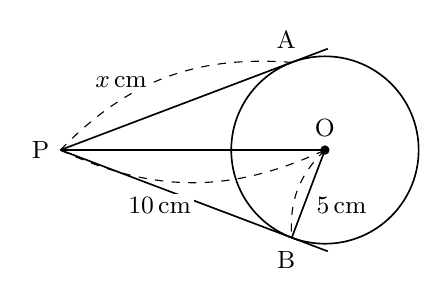
\begin{tikzpicture}[scale=1.4, line width=0.6pt]
  \draw (0.900,0.000) circle (0.850);
  \fill (0.900,0.000) circle (1.2pt);
  \draw (-1.500,0.000) -- (0.926,0.919);
  \draw (-1.500,0.000) -- (0.926,-0.919);
  \draw (-1.500,0.000) -- (0.900,0.000);
  \draw (0.900,0.000) -- (0.599,-0.795);
  \draw[dashed, line width=0.4pt] (-1.500,0.000) to[bend left=25] (0.599,0.795);
  \node[font=\small, fill=white, inner sep=1pt] at (-0.950,0.620) {$x\,\mathrm{cm}$};
  \draw[dashed, line width=0.4pt] (-1.500,0.000) to[bend right=25] (0.900,0.000);
  \node[font=\small, fill=white, inner sep=1pt] at (-0.600,-0.500) {$10\,\mathrm{cm}$};
  \draw[dashed, line width=0.4pt] (0.900,0.000) to[bend right=25] (0.599,-0.795);
  \node[font=\small, fill=white, inner sep=1pt] at (1.050,-0.500) {$5\,\mathrm{cm}$};
  \node[font=\small, inner sep=1.5pt] at (0.900,0.200) {O};
  \node[font=\small, inner sep=1.5pt] at (-1.680,0.000) {P};
  \node[font=\small, inner sep=1.5pt] at (0.549,0.995) {A};
  \node[font=\small, inner sep=1.5pt] at (0.549,-0.995) {B};
\end{tikzpicture}
